%%%%%%%%%%%%%%%%%%%%%%%%%%%%%%%%%%%%%%%%%%%%%%%%%
%%%%%%%%%%%%%%%%%%%%%%%%%%%%%%%%%%%%%%%%%%%%%%%%%

\chapter{Experimental Setup}
\label{chap:third}

%%%%%%%%%%%%%%%%%%%%%%%%%%%%%%%%%%%%%%%%%%%%%%%%%
%%%%%%%%%%%%%%%%%%%%%%%%%%%%%%%%%%%%%%%%%%%%%%%%%

%The same structure as before, including section, subsections and sub-subsections. Make sure that you follow the same conventions throughout, to avoid confusing the reader. Always remember to include a summary.

%%%%%%%%%%%%%%%%%%%%%%%%%%%%%%%%%%%%%%%%%%%%%%%%%
%%%%%%%%%%%%%%%%%%%%%%%%%%%%%%%%%%%%%%%%%%%%%%%%%

%Parameter
\section{Parameters}
\label{parameters}

For each class of environment, the following configurations were tested: The environment grid size, $S=50,100,200,300, 500$ where $S$ is the width and length of the grid and the percentage $p$ of the grid covered by objects, with $p= 5\%$, $20\%$, $50\%$, $70\%$, $90\%$. The ratio of prioritized to non-prioritized items $r$, is varied, where $r=0$, $0.2$,$0.25$, $0.333$, $0.5$, $0.667$, $0.75$, $0.8$, $1$. Honey bee specific parameters were selected based on \cite{seeley2009wisdom} as 
$t_{max}=200$ time steps, $f_{max}=100$ time steps, $\phi=0.8$ and $\rho=0.1$.

For all algorithms, robots were initially configured to forage either the prioritized item or the non-prioritized item with a ratio of $\tau=0$, $0.2$, $0.25$, $0.333$, $0.5$, $0.667$, $0.75$, $0.8$,$1$. Different numbers of robots, $c$, were used with $c=10, 30, 50, 70, 100$; $c$ is defined as the percentage of cells of the grid size $S$ that are occupied by robots.

All agents begin at random positions adjacent to the sink in the exploration state. All algorithms were run for 10000 time steps, where an agent can move maximum 1 grid cell at a time, to any adjacent cell, with no stopping conditions. For all algorithms, the agents begin randomly positioned next to the sink. The beacon locating of the sinks is simulated by each agent evaluating and moving up a light intensity gradient. The colour of the light is used to distinguish between the 2 sinks.

\section{Performance Measures}
\label{thri:third:performancemeasures}

%What do I need to add to 
%TODO: The idea is to add more robots foraging the prioritized items.
The following performance measures were used: the percentage of each item foraged over time, average time a robot spent in waiting state, and the entropy of robot movement. Due to space constraints, only the percentage, $\sigma$, of prioritized items foraged is presented. 

	\begin{itemize}
		\item	Amount gold items foraged over time
		\item	Amount waste items foraged over time
		\item	Average distance each robot moves
		\item	Average Time to forage an item for all robots
		\item	Average time to locate an item for all robots
		\item	Average time to return an item for all robots
		\item	Entropy of robot movement
	\end{itemize}
	
%%%%%%%%%%%%%%%%%%%%%%%%%%%%%%%%%%%%%%%%%%%%%%%%%

\section{Environment Types}
\label{thri:third:environmenttypes}
Each environment type was chosen to examine specific capabilities of the algorithms. A uniformly distributed environment 

Four different classes of environments were used as follows:
\begin{enumerate}
\item Environments where items of each type are uniformly distributed (Fig \ref{fig:uniformenv}). The uniformly distributed environment is used as a base line to test the algorithms. A hypothesis is that the algorithms without memory or communication will perform better in the uniformly distributed environment. 
\item Clustered environments with clusters of item types generated by randomly relabelling items in clusters generated by Lumer-Faieta ant cemetery clustering \cite{lumer1994diversity} as either prioritized or non-prioritized items (Fig \ref{fig:clusterenv}). These algorithms test the algorithms ability to exploit good areas. It will also test how algorithm can move past non-prioritized items. 
\item Vein environments resembling the natural occurrence of gold \cite{frimmel2002recent} (Fig \ref{fig:veinenv}). The vein environments will test whether an algorithm can move along the lines created by the vein. 
\item Gaussian environments where prioritized items are focused at the environment center. (Fig \ref{fig:gaussianenv}). These environments are used to specifically examine how an algorithm can deal with moving past non-prioritized items to reach prioritized items. 
\end{enumerate} 

\vspace{-2em}
\begin{figure} [h]
        \centering
        \begin{subfigure}[b]{0.21\textwidth}
                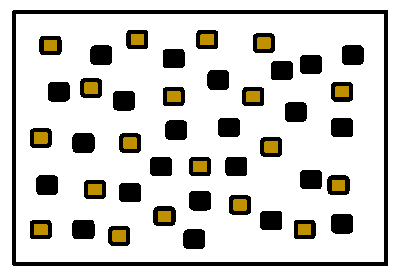
\includegraphics[width=\textwidth]{chapters/chapter4/figures/uniformenv.pdf}
                \caption{Uniform}
                \label{fig:uniformenv}
        \end{subfigure}%
        \begin{subfigure}[b]{0.205\textwidth}
                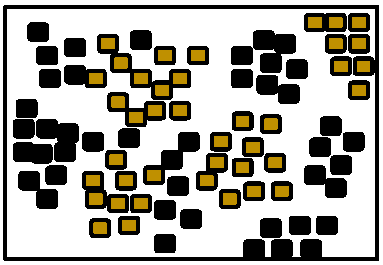
\includegraphics[width=\textwidth]{chapters/chapter4/figures/clusterenv.pdf}
                \caption{Clustered}
                \label{fig:clusterenv}
        \end{subfigure}
        \begin{subfigure}[b]{0.2\textwidth}
                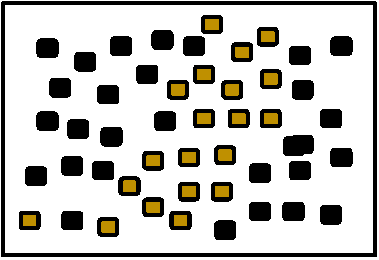
\includegraphics[width=\textwidth]{chapters/chapter4/figures/veinenv.pdf}
                \caption{Vein}
                \label{fig:veinenv}
        \end{subfigure}  
        \begin{subfigure}[b]{0.2\textwidth}
                        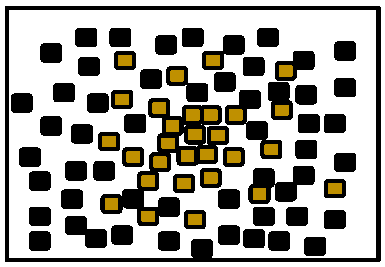
\includegraphics[width=\textwidth]{chapters/chapter4/figures/gaussianenv}
                        \caption{Gaussian}
                        \label{fig:gaussianenv}
       \end{subfigure}
        \caption{Environment Classes}\label{fig:environments}
\end{figure}


%%%%%%%%%%%%%%%%%%%%%%%%%%%%%%%%%%%%%%%%%%%%%%%%%
%%%%%%%%%%%%%%%%%%%%%%%%%%%%%%%%%%%%%%%%%%%%%%%%%
\section{Summary}
\label{fourth:summary}

%%%%%%%%%%%%%%%%%%%%%%%%%%%%%%%%%%%%%%%%%%%%%%%%%
%%%%%%%%%%%%%%%%%%%%%%%%%%%%%%%%%%%%%%%%%%%%%%%%%